\documentclass[noauthor,nooutcomes,12pt,handout,hints]{ximera}

\graphicspath{  
{./}
{./whoAreYou/}
{./drawingWithTheTurtle/}
{./bisectionMethod/}
{./circles/}
{./anglesAndRightTriangles/}
{./lawOfSines/}
{./lawOfCosines/}
{./plotter/}
{./staircases/}
{./pitch/}
{./qualityControl/}
{./symmetry/}
{./nGonBlock/}
}


%% page layout
\usepackage[cm,headings]{fullpage}
\raggedright
\setlength\headheight{13.6pt}


%% fonts
\usepackage{euler}

\usepackage{FiraMono}
\renewcommand\familydefault{\ttdefault} 
\usepackage[defaultmathsizes]{mathastext}
\usepackage[htt]{hyphenat}

\usepackage[T1]{fontenc}
\usepackage[scaled=1]{FiraSans}

%\usepackage{wedn}
\usepackage{pbsi} %% Answer font


\usepackage{cancel} %% strike through in pitch/pitch.tex


%% \usepackage{ulem} %% 
%% \renewcommand{\ULthickness}{2pt}% changes underline thickness

\tikzset{>=stealth}

\usepackage{adjustbox}

\setcounter{titlenumber}{-1}

%% journal style
\makeatletter
\newcommand\journalstyle{%
  \def\activitystyle{activity-chapter}
  \def\maketitle{%
    \addtocounter{titlenumber}{1}%
                {\flushleft\small\sffamily\bfseries\@pretitle\par\vspace{-1.5em}}%
                {\flushleft\LARGE\sffamily\bfseries\thetitlenumber\hspace{1em}\@title \par }%
                {\vskip .6em\noindent\textit\theabstract\setcounter{question}{0}\setcounter{sectiontitlenumber}{0}}%
                    \par\vspace{2em}
                    \phantomsection\addcontentsline{toc}{section}{\thetitlenumber\hspace{1em}\textbf{\@title}}%
                     }}
\makeatother



%% thm like environments
\let\question\relax
\let\endquestion\relax

\newtheoremstyle{QuestionStyle}{\topsep}{\topsep}%%% space between body and thm
		{}                      %%% Thm body font
		{}                              %%% Indent amount (empty = no indent)
		{\bfseries}            %%% Thm head font
		{)}                              %%% Punctuation after thm head
		{ }                           %%% Space after thm head
		{\thmnumber{#2}\thmnote{ \bfseries(#3)}}%%% Thm head spec
\theoremstyle{QuestionStyle}
\newtheorem{question}{}



\let\freeResponse\relax
\let\endfreeResponse\relax

%% \newtheoremstyle{ResponseStyle}{\topsep}{\topsep}%%% space between body and thm
%% 		{\wedn\bfseries}                      %%% Thm body font
%% 		{}                              %%% Indent amount (empty = no indent)
%% 		{\wedn\bfseries}            %%% Thm head font
%% 		{}                              %%% Punctuation after thm head
%% 		{3ex}                           %%% Space after thm head
%% 		{\underline{\underline{\thmname{#1}}}}%%% Thm head spec
%% \theoremstyle{ResponseStyle}

\usepackage[tikz]{mdframed}
\mdfdefinestyle{ResponseStyle}{leftmargin=1cm,linecolor=black,roundcorner=5pt,
, font=\bsifamily,}%font=\wedn\bfseries\upshape,}


\ifhandout
\NewEnviron{freeResponse}{}
\else
%\newtheorem{freeResponse}{Response:}
\newenvironment{freeResponse}{\begin{mdframed}[style=ResponseStyle]}{\end{mdframed}}
\fi



%% attempting to automate outcomes.

%% \newwrite\outcomefile
%%   \immediate\openout\outcomefile=\jobname.oc
%% \renewcommand{\outcome}[1]{\edef\theoutcomes{\theoutcomes #1~}%
%% \immediate\write\outcomefile{\unexpanded{\outcome}{#1}}}

%% \newcommand{\outcomelist}{\begin{itemize}\theoutcomes\end{itemize}}

%% \NewEnviron{listOutcomes}{\small\sffamily
%% After answering the following questions, students should be able to:
%% \begin{itemize}
%% \BODY
%% \end{itemize}
%% }
\usepackage[tikz]{mdframed}
\mdfdefinestyle{OutcomeStyle}{leftmargin=2cm,rightmargin=2cm,linecolor=black,roundcorner=5pt,
, font=\small\sffamily,}%font=\wedn\bfseries\upshape,}
\newenvironment{listOutcomes}{\begin{mdframed}[style=OutcomeStyle]After answering the following questions, students should be able to:\begin{itemize}}{\end{itemize}\end{mdframed}}



%% my commands

\newcommand{\snap}{{\bfseries\itshape\textsf{Snap!}}}
\newcommand{\flavor}{\link[\snap]{https://snap.berkeley.edu/}}
\newcommand{\mooculus}{\textsf{\textbf{MOOC}\textnormal{\textsf{ULUS}}}}


\usepackage{tkz-euclide}
\tikzstyle geometryDiagrams=[rounded corners=.5pt,ultra thick,color=black]
\colorlet{penColor}{black} % Color of a curve in a plot



\ifhandout\newcommand{\mynewpage}{\newpage}\else\newcommand{\mynewpage}{}\fi


\title{Symmetries of the regular triangle}

\author{Bart Snapp}

\begin{document}
\begin{abstract}
  Something
\end{abstract}
\maketitle

\begin{listOutcomes}
\item Witness the symmetries of the regular triangle.
\item Describe symmetries of the regular triangle.
\item Think of the symmetries of the regular triangle as functions.
\item Compose these functions and use \snap\ to show the result.
\end{listOutcomes}
\mynewpage


\begin{question}
  The symmetries of the regular triangle are those that leave it
  unchanged. To see these symmetries, it is helpful to color-in the
  sides of the triangle. For example, here is a symmetry of the
  regular triangle:
  \[
  \raisebox{-.4\height}{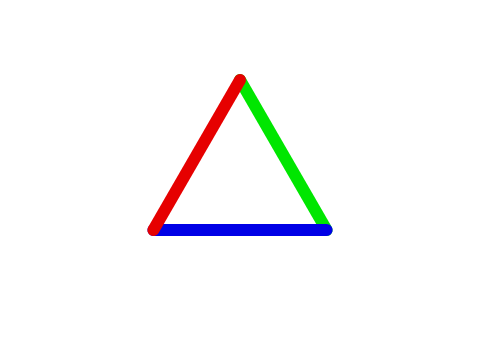
\includegraphics[width=2.5in]{eTri.png}}\resizebox{.7in}{!}{$\mapsto$} \raisebox{-.4\height}{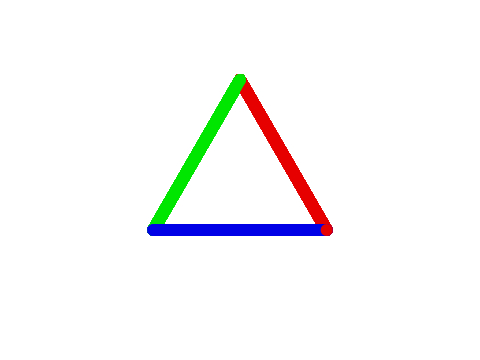
\includegraphics[width=2.5in]{rfTri.png}}
  \]
  Use \snap\ to make STAGES for each symmetry of the regular triangle,
  and display them as a function as I did above.
\end{question}
\mynewpage

\begin{question}
  Let $r$ be a clockwise $120^\circ$ rotation about the center of the
  triangle. Let $f$ be a flip across a vertical line down the middle
  of the triangle. Find pictures representing:
  \begin{enumerate}
  \item $r$
  \item $r^2$
  \item $f$
  \item $SF$
  \item $r^2 f$.
  \end{enumerate}
  In each case, show off your work by displaying your SCRIPT and
  STAGE.
  \begin{hint}
    Note, when looking at something like $rf$, first we flip the
    triangle, then we rotate it. 
  \end{hint}
\end{question}
\mynewpage


\begin{question}
  Do you remember the MULTIPLICATION TABLES? We can make a similar
  table for symmetries of regular triangles. Here, I've started it for
  you:
  \[
  \begin{array}{|c||c|c|c|c|c|c|}
    \hline
      & e & r & r^2 & f & rf & r^2f\\ \hline\hline
    e & e & r & r^2 & f & rf & r^2f\\ \hline
    r & r & r^2 & \color{red}r^3 & rf & r^2f & \color{red}r^3f\\ \hline
    r^2 & r^2 & \color{red}r^3 & \color{red}r^4 & r^2f & \color{red}r^3f &\color{red} r^4f\\ \hline
    f  & f & \color{red}fr & \color{red}fr^2 & \color{red}f^2 & \color{red}frf & \color{red}fr^2f\\ \hline
    rf & rf & \color{red}rfr & \color{red}rfr^2 & \color{red}rf^2 & \color{red}rfrf & \color{red}rfr^2f\\ \hline
    r^2f & r^2f & \color{red}r^2fr & \color{red}r^2fr^2 & \color{red}r^2f^2 &\color{red} r^2frf &\color{red} r^2fr^2f\\ \hline
  \end{array}
  \]
  Each of the symmetries in red is actually equal to one of the
  symmetries in top row (or left-most column)
  \[
  e,\quad r,\quad r^2,\quad f,\quad rf,\quad r^2f
  \]
  where $e$ is the ``do-nothing'' symmetry. EXPRESS each of the red
  symmetries as one of $e,r,r^2,f,rf,r^2f$ and UPDATE the table with
  these values.
\end{question}
\end{document}
